\documentclass{article}
\usepackage[utf8]{inputenc}
\usepackage{titling}
\usepackage{graphicx}
\usepackage{xcolor}
\usepackage[colorlinks=true,linkcolor=darkgray, urlcolor =gray]{hyperref}
\usepackage[spanish]{babel}
\DeclareUnicodeCharacter{301}{~}
\usepackage{url}


\title{Práctica 6. Introducción al aprendizaje computacional con WEKA}
\author{Cristina Díaz García}
\date{Abril 2019}

\renewcommand\maketitlehooka{\null\mbox{}\vfill}
\renewcommand\maketitlehookd{\vfill\null}


\begin{document}

\addcontentsline{toc}{section}{Índice general}

\begin{titlingpage}
\maketitle
\end{titlingpage}

\newpage

\tableofcontents

\newpage

\section{Enunciado}

\textbf{\underline{Tarea:}} Contesta a las preguntas que figuran a continuación.

\textbf{\underline{Entrega:}} Documento pdf con la solución (capturas de pantalla y textos descriptivos).

\section{Pregunta 1}

¿Cómo clasificaríamos a un bicho rojizo que cojea según este modelo? ¿Y a un bicho de piel escamosa? ¿Y a un bicho de piel suave, rojizo y con cuatro patas?

\subsection{Solución proporcionada}

Usando el árbol proporcionado:

\begin{center}
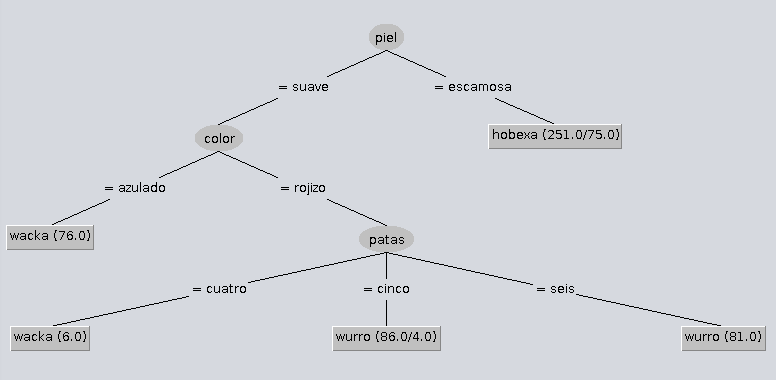
\includegraphics[scale=0.5]{images/tree.png}
\end{center}

\begin{itemize}
\item \textbf{Bicho rojizo que cojea:} En la primera decisión no tenemos información suficiente, así que con este modelo, no se podría clasificar este ejemplo.
\item \textbf{Bicho de piel escamosa:} En la primera decisión, llegamos a la determinación de que es un hobexa.
\item \textbf{Bicho de piel suave, rojizo y con cuatro patas:} En la primera decisión, tomaríamos el camino de la piel suave, llegando a la decisión del color de piel, que como es rojizo, necesitamos el número de patas, que al ser 4, el resultado es wacka.
\end{itemize}

\section{Pregunta 2}

¿Encuentras alguna explicación razonable a que los errores de clasificación se cometan con las wackas?

\subsection{Solución proporcionada}

Porque de los wackas es de los que menos información segura tenemos: ninguno de sus atributos son indistinguiblemente suyos.

\section{Pregunta 3}

¿Cómo clasificaríamos a un bicho rojizo que cojea según este modelo? ¿Y a un bicho de piel escamosa? ¿Y a un bicho de piel suave, rojizo y con cuatro patas?

\subsection{Solución proporcionada}

Usando las reglas proporcionadas:

\begin{center}
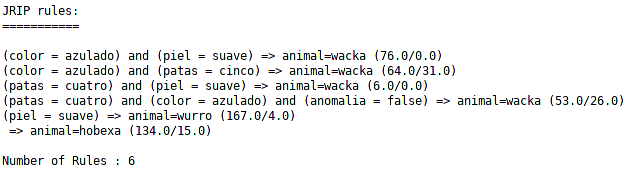
\includegraphics[scale=0.5]{images/rules.png}
\end{center}

\begin{itemize}
\item \textbf{Bicho rojizo que cojea:} Como no cumple ninguna de las reglas con condiciones, pasaría por la sexta regla, por lo que se clasificaría como hobexa.
\item \textbf{Bicho de piel escamosa:} Como no cumple ninguna de las reglas con condiciones, pasaría por la sexta regla, por lo que se clasificaría como hobexa.
\item \textbf{Bicho de piel suave, rojizo y con cuatro patas:} Cumple la tercera regla, por lo que se clasificaría como un wacka.
\end{itemize}

\section{Pregunta 4}

¿Cuántos varones viajaban en el Titanic? ¿Cuántas mujeres? ¿Cuántos menores de edad? ¿Cuántos
viajeros en primera clase? Modifica los parámetros del algoritmo para que aprenda 26 reglas de asociación con una confianza de 0.85, e interpreta el significado de las cinco últimas.

\subsection{Solución proporcionada}

\textbf{Clasificados por sexo}

\begin{center}
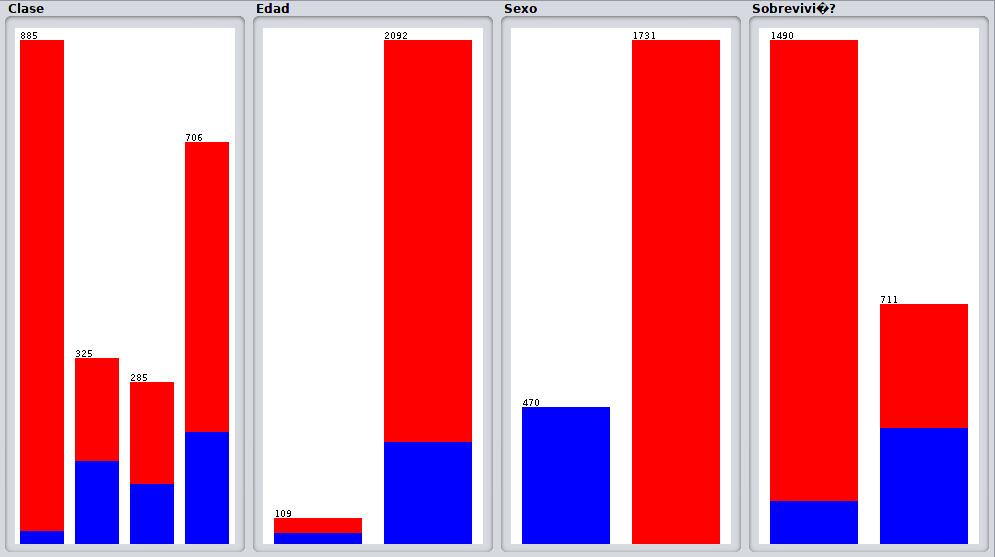
\includegraphics[scale=0.3]{images/sexo.png}
\end{center}

\textbf{Clasificados por edad}

\begin{center}
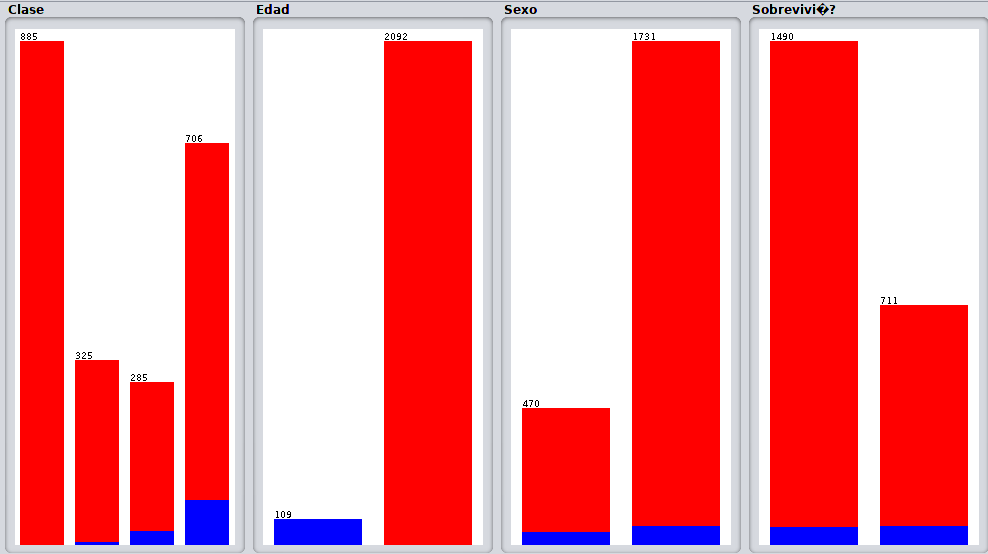
\includegraphics[scale=0.3]{images/edad.png}
\end{center}

\newpage

\textbf{Clasificados por clase}

\begin{center}
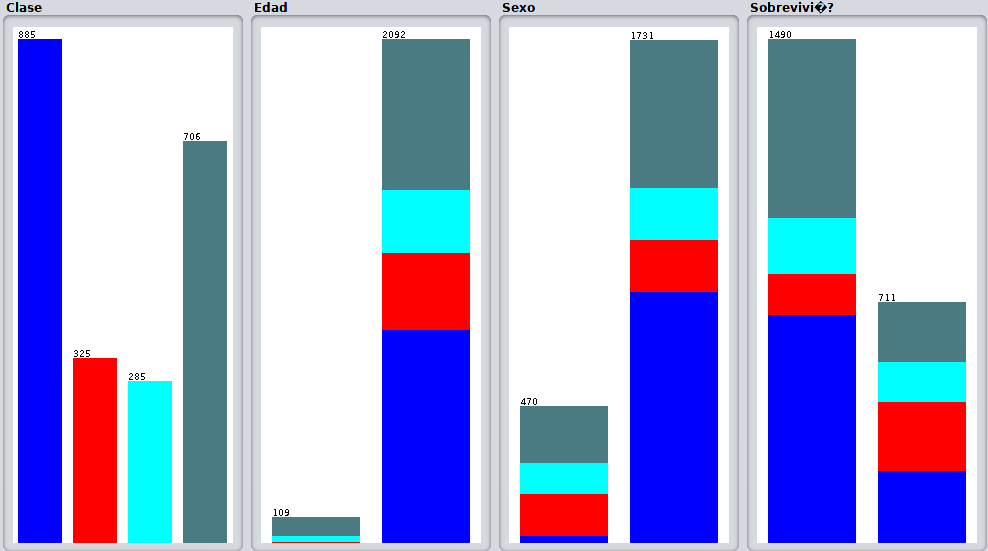
\includegraphics[scale=0.3]{images/clase.png}
\end{center}

\begin{itemize}
\item \textbf{Hombres que viajaban:} 1731
\item \textbf{Mujeres que viajaban:} 470
\item \textbf{Menores que viajaban:} 109
\item \textbf{Viajeros en primera clase:} 325
\end{itemize}

Esta es la salida inicial del algoritmo:

\begin{center}
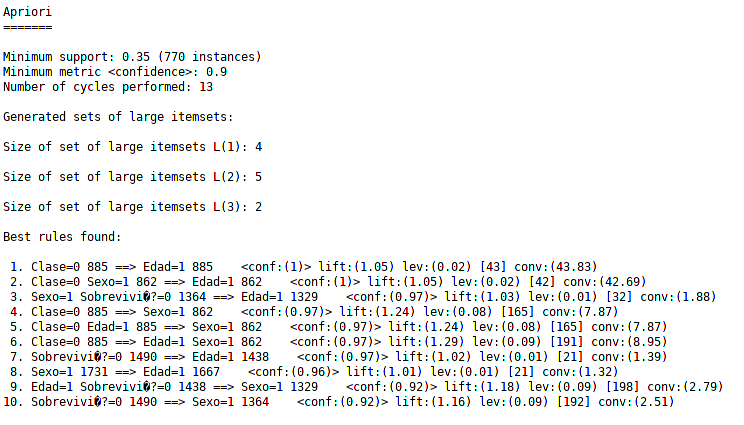
\includegraphics[scale=0.5]{images/titanic.png}
\end{center}

Tras modificar el algoritmo, el resultado es el siguiente:

\begin{center}
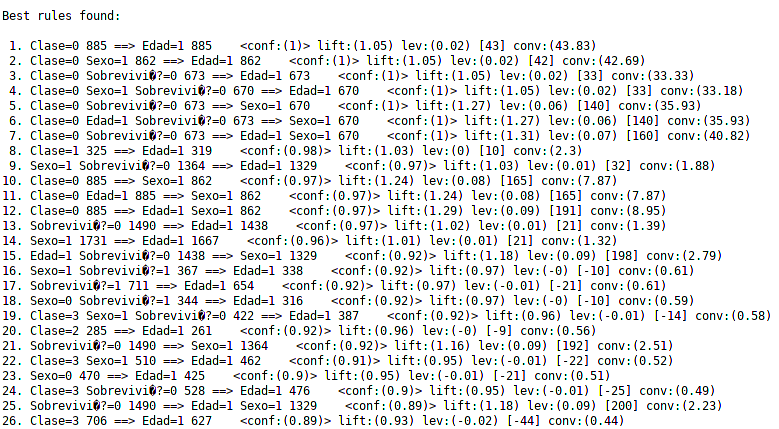
\includegraphics[scale=0.5]{images/mod.png}
\end{center}

\textbf{Regla 22}

La probabilidad de que la persona sea de tercera clase, hombre y que muriera es del 89\%.

\textbf{Regla 23}

La probabilidad de que la persona sea mujer y mayor de edad es del 90\%.

\textbf{Regla 24}

La probabilidad de que la persona sea de tercera clase, mayor de edad y que muriera es del 90\%.

\textbf{Regla 25}

La probabilidad de que la persona hombre mayor de edadd y muriera es del 89\%.

\textbf{Regla 26}

La probabilidad de que la persona sea de tercera clase y mayor de edad es del 89\%.

\section{Pregunta 5}

A la vista de los datos relativos a cada cluster, ¿qué grupo crees que representa mejor a los
estudiantes que van a aprobar la asignatura? ¿Y a los que van a suspenderla?

\subsection{Solución proporcionada}

Esta es la salida del algoritmo:

\begin{center}
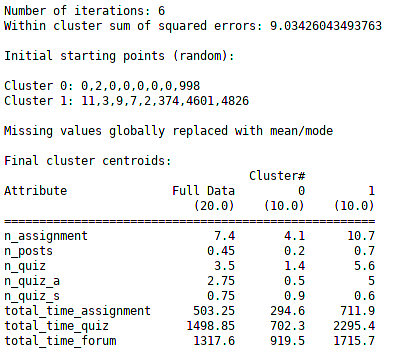
\includegraphics[scale=0.5]{images/cluster.png}
\end{center}

Ya que los resultados son mayores en el segundo cluster (Cluster \#1), se podría pensar que es el que mejor representa a los estudiantes que aprobarán, siendo el primer cluster (Cluster \#0), el de los estudiantes que suspenderán.

\begin{thebibliography}{9}
\bibitem{Bayes} Información oficial de GeNIe, \url{https://www.bayesfusion.com}.
\end{thebibliography}

\end{document}